\section{Analysis}
\label{sec:analysis}
%(2 pages)

As noted previously, progress on knowledge base population has been slow and arduous.
Let's proceed with an analysis of submissions and evaluations thus far, with the motivation of identifying potential obstacles for system development. 

\paragraph{Data.}
We will make use of system submissions released as part of the TAC-KBP Slot Validation tracks in 2013, 2014 and 2015.
The 2015 dataset contains 70 submissions from 18 teams for 317 queries.
Considering only the submissions to the first hop of the two-hop evaluation,
each submission contains on average about 35,951 predicted slotfills. 
There are in total 201,332 relations that were predicted, of which only 11,008 of these slotfills have were evaluated.

% NOTE: should we describe any more statistics?

\begin{figure*}
  \begin{subfigure}{0.49\textwidth}
  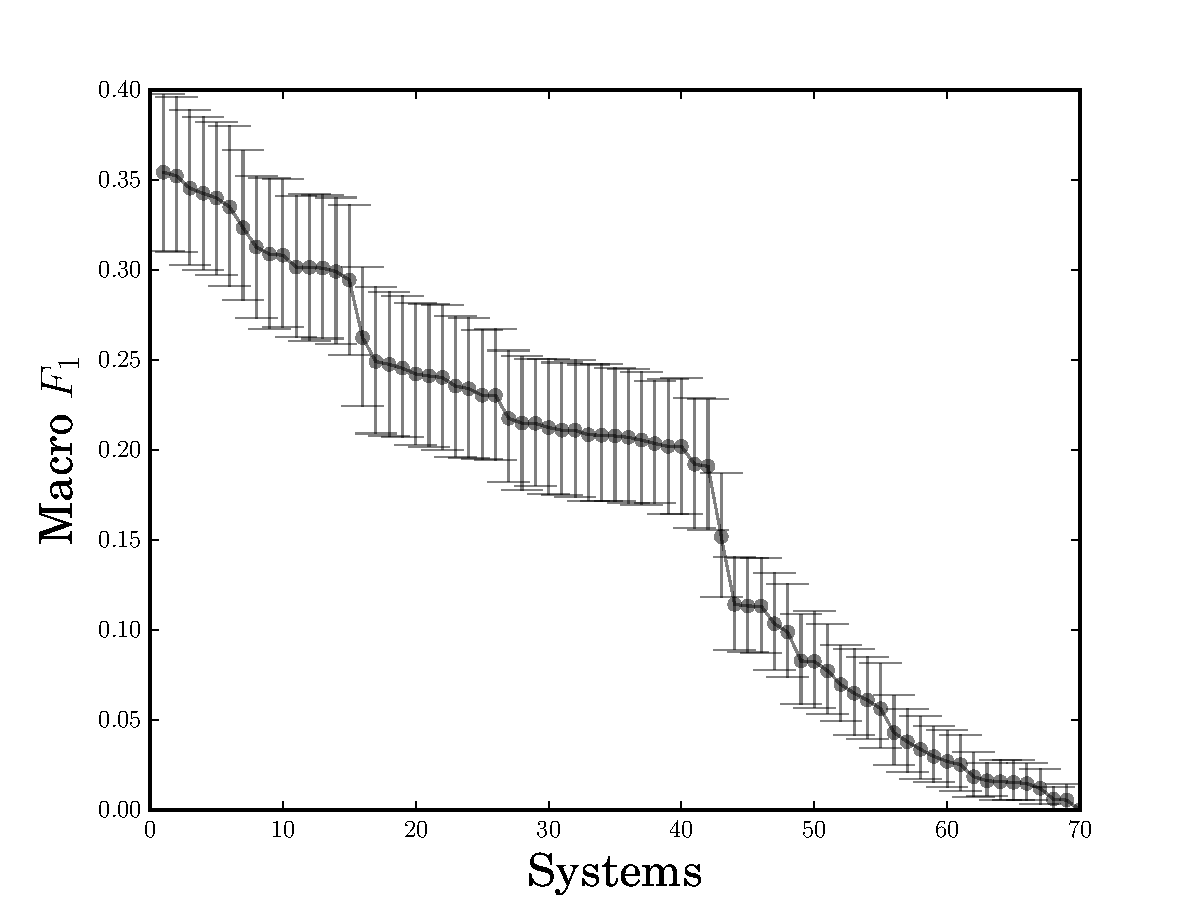
\includegraphics[width=\columnwidth]{figures/experiment1}
  \caption{\label{fig:f1}}
  \end{subfigure}
  \begin{subfigure}{0.49\textwidth}
  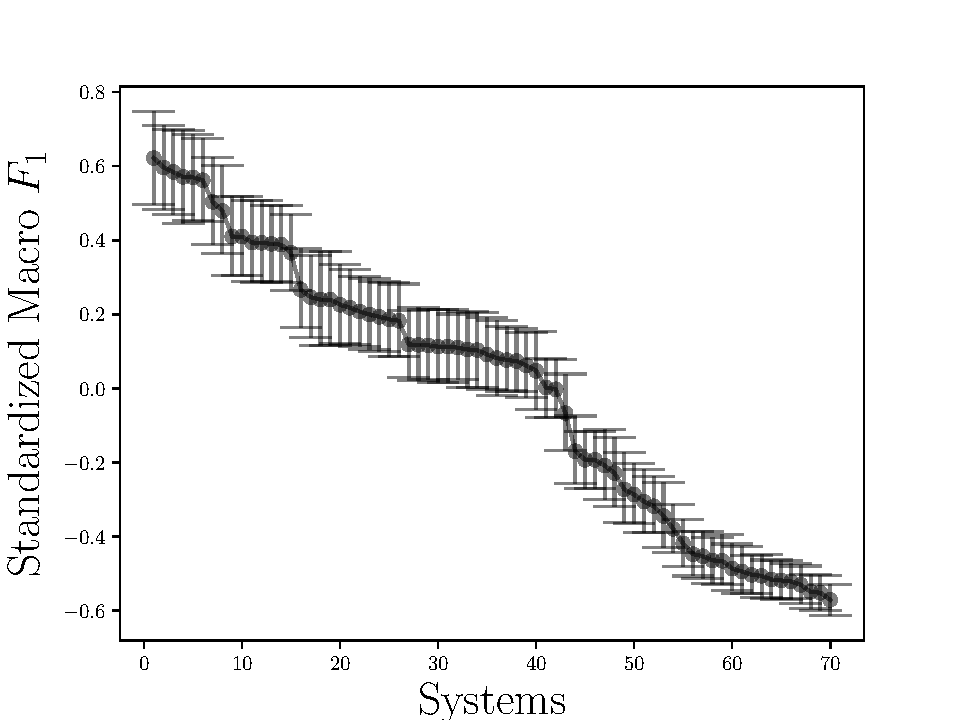
\includegraphics[width=\columnwidth]{figures/experiment3}
  \caption{\label{fig:sf1}}
  \end{subfigure}
  \caption{}
\end{figure*}

\begin{table}
  \begin{tabular} {l r r r r} \toprule
    Metric & \multicolumn{2}{c}{Normal} & \multicolumn{2}{c}{Standardized} \\
              Average value & 95\% confidence interval & Mean difference between top 10 teams &  Average value & 95\% confidence interval  \\  \midrule 
Micro $P^e$     & $30.91\%$ &  $16.77\%$ & 0.12\% &     &  \\
Micro $R^e$     & $30.45\%$ &  $ 6.41\%$ & 0.17\% &     &  \\
Micro $\fone^e$ & $38.62\%$ &  $ 6.79\%$ & 0.24\% &     &  \\
Macro $P^e$     & $24.98\%$ &  $ 6.93\%$ & 0.24\% &     &  \\
Macro $R^e$     & $03.56\%$ &  $ 6.87\%$ & 0.23\% &     &  \\
Macro $\fone^e$ & $22.72\%$ &  $ 6.19\%$ & 1.04\% &     &  \\ \bottomrule
  \end{tabular}






  \caption{\label{metric-variance}}
\end{table}

\paragraph{How informative is \fone{} as a metric?}
Most teams hill climb on a combination of micro and macro entity-level $\fone$ during development.
It is natural to ask how much of an improvement on the metric score is necessary to actually trust that system performance has improved.
We use a bootstrap sampling method to estimate the variance of $\fone$ and other metrics over query sets \tableref{metric-variance} and measure the 95\% confidence intervals for system scores \figureref{f1}.
The median difference in metric scores between adjacent submissions in the top 10 scores (for that metric) is between 0.1--1\%,
while the confidence intervals are at least 6\%.
% TODO: we can use the differences between the submissions of the each team.
It is hard for the researcher to identify if any of the presumably distinct submissions hold any water of another.

Next, we would like to ask what factors contribute to the large variance in the system metrics above.
One natural confounding variable is the substantial variability in the difficulty of query entities.
We can measure the effect of the query entity by analyzing the variation in topic-model scores.
Consider the linear model,
\begin{align*}
  X_{s,e} &= \mu 
    + \underbrace{\mu_{s} - \mu}_{\nu_{s}}
    + \underbrace{\mu_{e} - \mu}_{\nu_{e}}
    + \underbrace{X_{s,e} - \nu_{s} - \nu_{e} - \mu}_{\nu_{s,e}},
\end{align*}
where $\nu_{s}$, $\nu_{e}$ and $\nu_{s,e}$ capture the effect of the system $s$ and query entity $e$, and the residual.
Variance can also be decomposed as,
\begin{align*}
  \sigma^2(X_{s,e}) &= \sigma^2(\nu_s) + \sigma^2(\nu_e) + \sigma^2(\nu_{s,e}).
\end{align*}

\begin{tabular}{l r r r r r}
  Metric & $\sigma$ & $\sigma_{s}$ & $\sigma_{e}$ & $\sigma_{s,e}$ \\
\fone& 0.101898302295&0.012239521201&0.0212129246589&0.0684458564356&0.120115064974&0.151694415512
\end{tabular}

\tableref{} shows the variance explained by different components for macro metrics. As we can see, almost twice as much of the variance is explained by the entity only as that of the system.
% Explain what the high q,e scores mean.
%Another consequence is in confidence intervals.
%Bad differentiation from pairwise scores.

\paragraph{Controlling for query variance.}

It's easy for us to control for query variance by standardizing our metric,  
$$X'_{se} = \frac{X_{se} - \mu_e}{\sigma_e}$$.

\figureref{sf1} plots the performance of systems under the standardized macro \fone metric.
% TODO: variance under standardized metric -- showing less contribution
% due to queries and an overall reduction in variance.
% NOTE: This is only useful when comparing systems, as one is wont to do during development.

% TODO: I wish we could give scroes for this.
% \subsection{Are we improving over time?}

\subsection{What is the effect of pooling?}

\begin{figure}
  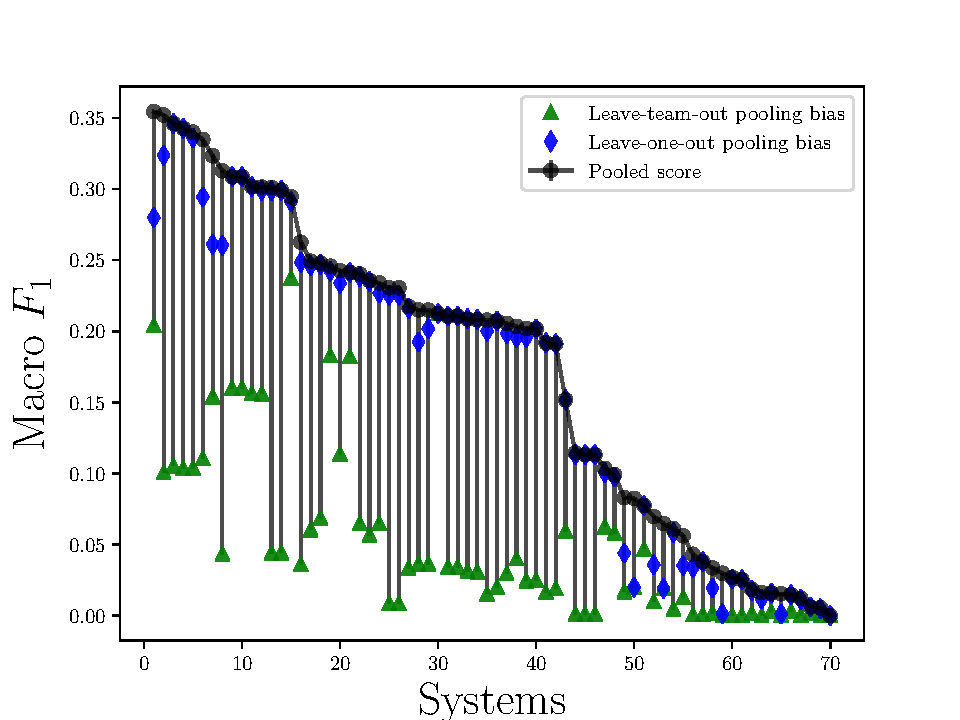
\includegraphics[width=\columnwidth]{figures/experiment2}
  \caption{Pooling bias.}
\end{figure}

Another aspect of the evaluation that could have adverse effects on system developments is the pooling approach used to collect contexts that contain mentions.
% While humans independently contribute to this pool, there j0

Define pooling bias. Statistical model used.
Significant!

If we increased the amount of data annotated, we may hopefully avoid pooling bias.
Expensive and perhaps regressive.
Next section, explore a new way.

